\documentclass[11pt,a4paper]{article}
\usepackage[T1]{fontenc}
\usepackage[utf8]{inputenc}
\usepackage[a4paper, margin=1.5cm]{geometry}
\usepackage{amsmath}
\usepackage{tikz}
\usepackage{float}
\usetikzlibrary{patterns, decorations.pathreplacing, calc, arrows.meta}

% Couleurs personnalisees
\definecolor{wpetg}{RGB}{34,139,34}
\definecolor{aircolor}{RGB}{200,230,255}
\definecolor{billeA}{RGB}{218,165,32}
\definecolor{billeB}{RGB}{205,92,92}
\definecolor{watercolor}{RGB}{100,180,255}
\definecolor{conecolor}{RGB}{255,200,100}

\pagestyle{empty}

\begin{document}

\begin{center}
{\Large\bfseries Coupe XZ -- Cone inscrit dans la cavite}\\[0.3cm]
{\large Demi-angle $\theta = 48.4$\textdegree}
\end{center}

\vspace{0.5cm}

\begin{center}
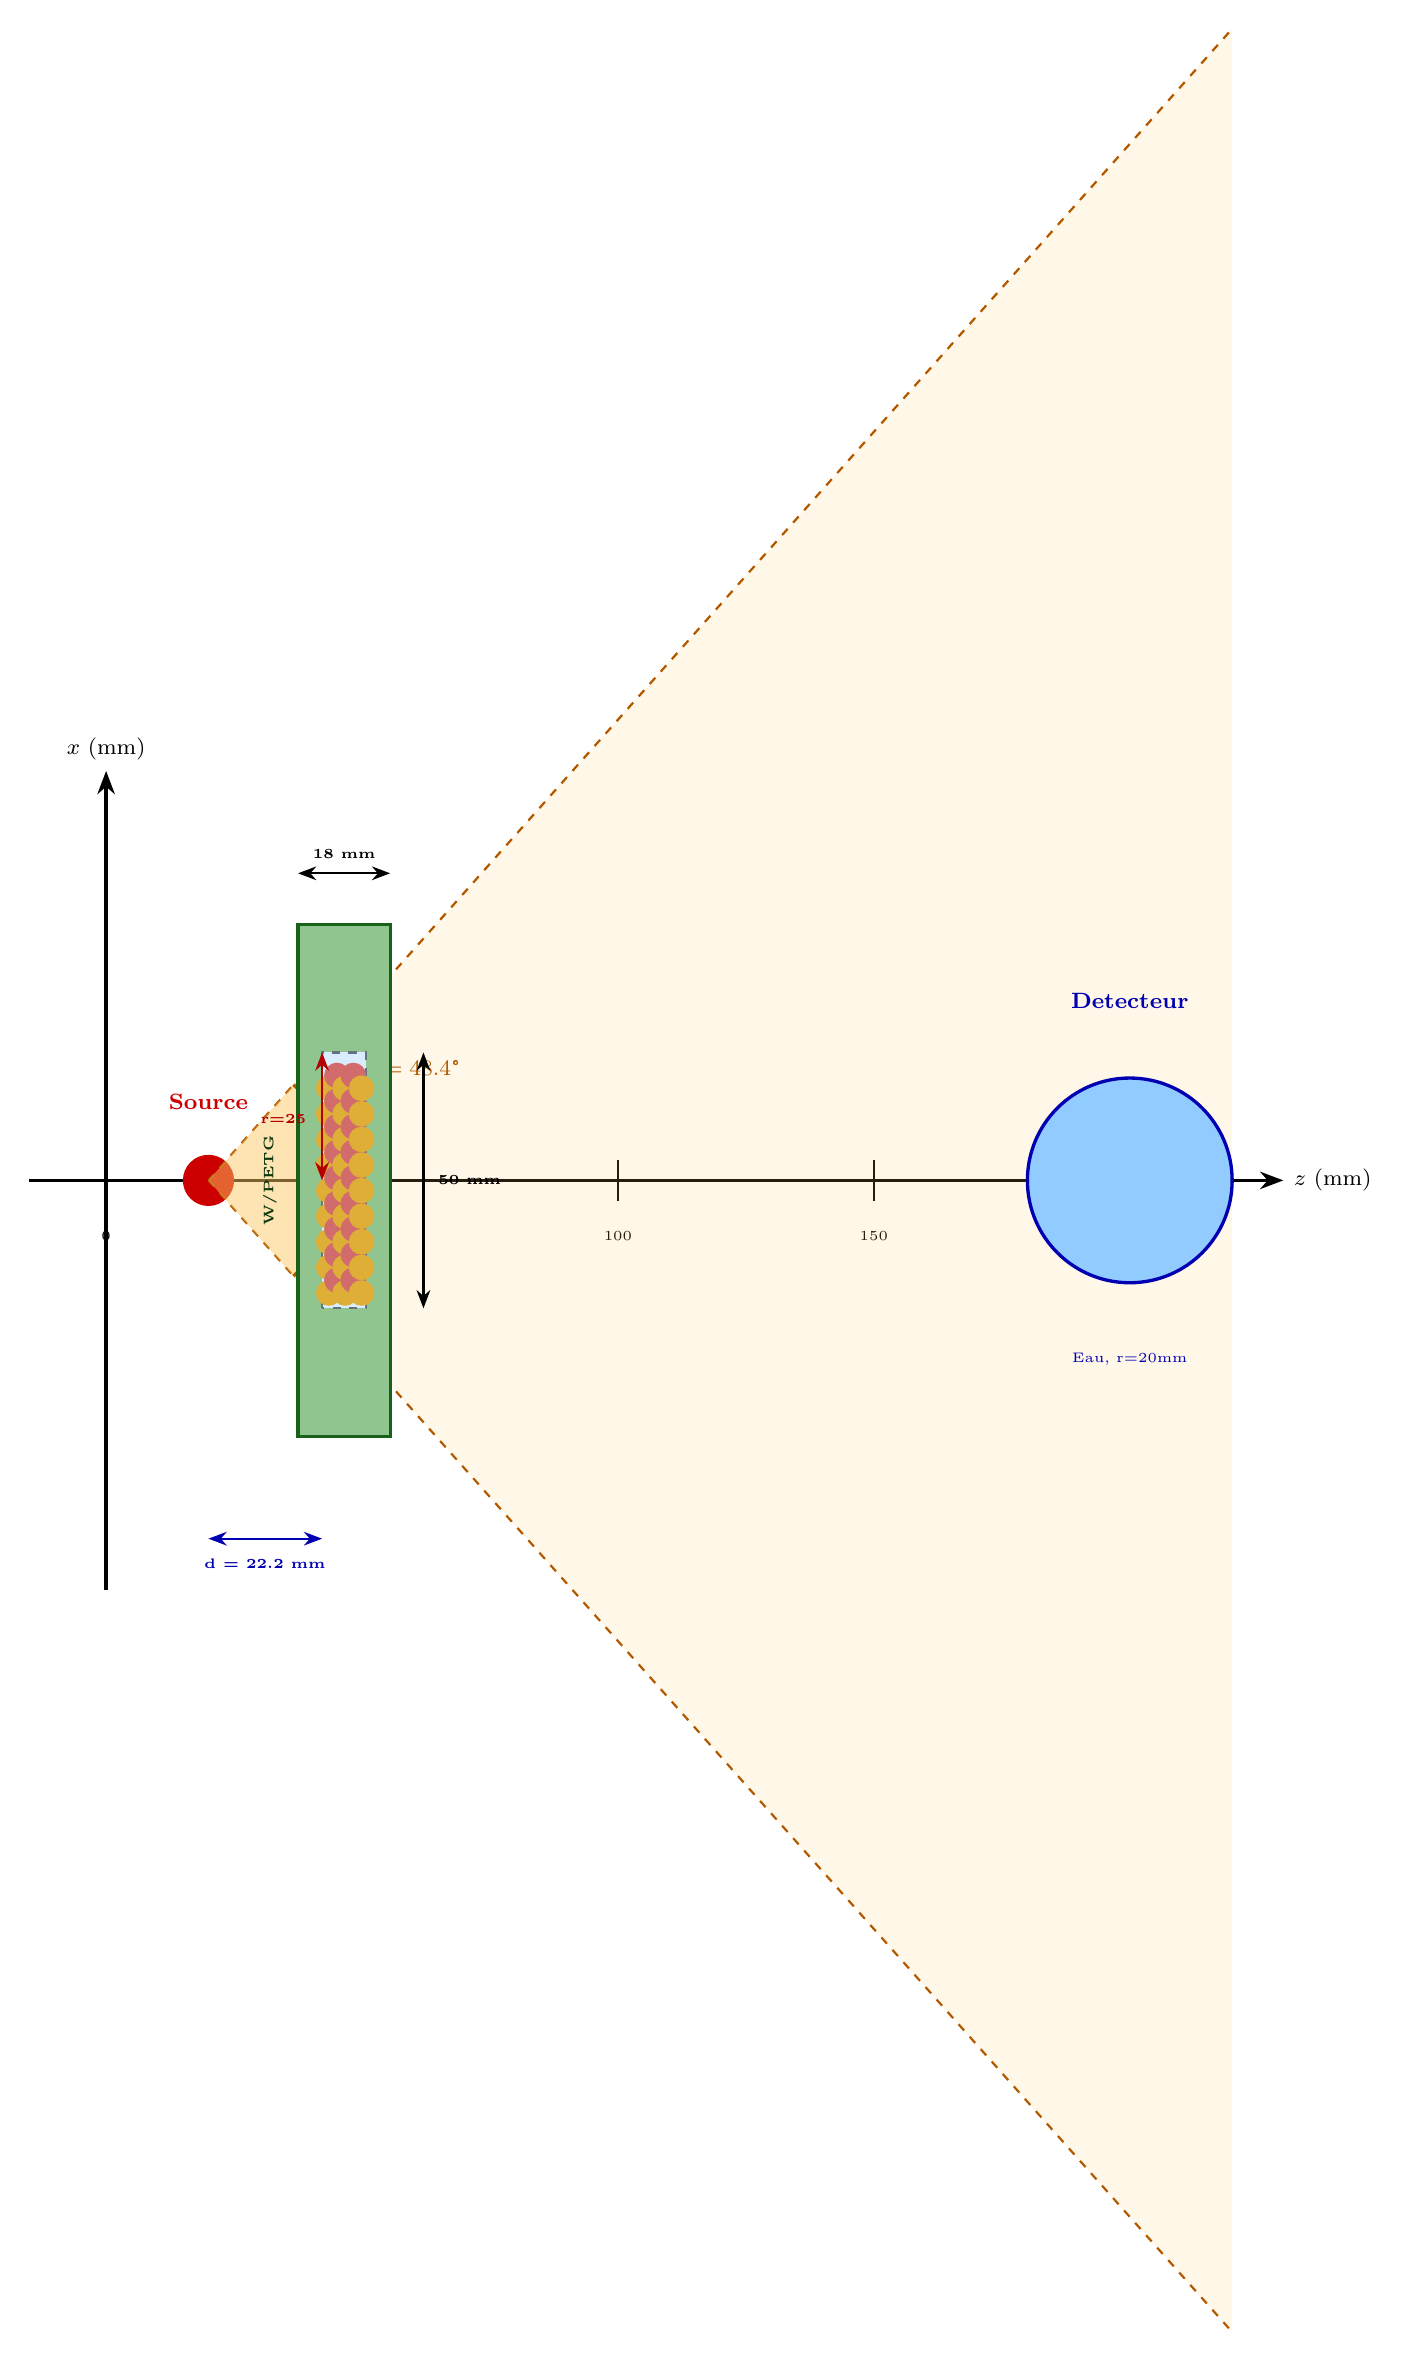
\begin{tikzpicture}[scale=0.065, >=Stealth]

% =============================================================================
% AXE Z (horizontal) et AXE X (vertical)
% =============================================================================
\draw[->, very thick] (-15, 0) -- (230, 0) node[right] {\footnotesize $z$ (mm)};
\draw[->, very thick] (0, -80) -- (0, 80) node[above] {\footnotesize $x$ (mm)};

% Graduations sur l'axe Z
\foreach \z in {0, 50, 100, 150, 200} {
    \draw[thick] (\z, -4) -- (\z, 4);
    \node[below, font=\tiny] at (\z, -8) {\z};
}

% =============================================================================
% SOURCE (z = 20 mm)
% =============================================================================
\fill[red!80!black] (20, 0) circle (5);
\node[above, red!80!black, font=\footnotesize\bfseries] at (20, 12) {Source};

% =============================================================================
% CONE DE DEMI-ANGLE 48.4 degres
% =============================================================================
% Cone colore jusqu'au detecteur
\fill[conecolor, opacity=0.15] (20, 0) -- (220, 225) -- (220, -225) -- cycle;

% Lignes du cone (bords)
\draw[orange!70!black, thick, dashed] (20, 0) -- (220, 225);
\draw[orange!70!black, thick, dashed] (20, 0) -- (220, -225);

% Cone jusqu'a la cavite (plus visible)
\fill[conecolor, opacity=0.4] (20, 0) -- (42.2, 25) -- (42.2, -25) -- cycle;

% Arc pour l'angle
\draw[orange!70!black, very thick] (20,0) ++(0:25) arc (0:48.4:25);
\draw[orange!70!black, very thick] (20,0) ++(0:25) arc (0:-48.4:25);
\node[orange!70!black, font=\footnotesize\bfseries] at (60, 22) {$\theta=48.4$\textdegree};

% =============================================================================
% PLAQUE W/PETG (z = 37.5 a 55.5 mm, x = -50 a +50 mm)
% =============================================================================
\fill[wpetg!50] (37.5, -50) rectangle (55.5, -25);
\fill[wpetg!50] (37.5, 25) rectangle (55.5, 50);
\fill[wpetg!50] (37.5, -25) rectangle (42.2, 25);
\fill[wpetg!50] (50.8, -25) rectangle (55.5, 25);

% Contour de la plaque
\draw[wpetg!70!black, very thick] (37.5, -50) rectangle (55.5, 50);

\node[wpetg!40!black, font=\tiny\bfseries, rotate=90] at (32, 0) {W/PETG};

% =============================================================================
% CAVITE D'AIR
% =============================================================================
\fill[aircolor!70] (42.2, -25) rectangle (50.8, 25);
\draw[aircolor!50!black, thick, dashed] (42.2, -25) rectangle (50.8, 25);
\node[font=\tiny] at (46.5, 0) {Air};

% =============================================================================
% BILLES DE BISMUTH (5 plans)
% =============================================================================
\def\r{2.5}

% Plan 1 (A)
\foreach \x in {-22, -17, -12, -7, -2, 3, 8, 13, 18} {
    \fill[billeA!90] (43.5, \x) circle (\r);
}
% Plan 2 (B)
\foreach \x in {-19.5, -14.5, -9.5, -4.5, 0.5, 5.5, 10.5, 15.5, 20.5} {
    \fill[billeB!90] (45.1, \x) circle (\r);
}
% Plan 3 (A)
\foreach \x in {-22, -17, -12, -7, -2, 3, 8, 13, 18} {
    \fill[billeA!90] (46.7, \x) circle (\r);
}
% Plan 4 (B)
\foreach \x in {-19.5, -14.5, -9.5, -4.5, 0.5, 5.5, 10.5, 15.5, 20.5} {
    \fill[billeB!90] (48.3, \x) circle (\r);
}
% Plan 5 (A)
\foreach \x in {-22, -17, -12, -7, -2, 3, 8, 13, 18} {
    \fill[billeA!90] (49.9, \x) circle (\r);
}

% =============================================================================
% DETECTEUR DOSE (z = 200 mm)
% =============================================================================
\fill[watercolor!70] (200, 0) circle (20);
\draw[blue!70!black, very thick] (200, 0) circle (20);
\node[blue!70!black, font=\footnotesize\bfseries] at (200, 35) {Detecteur};
\node[blue!70!black, font=\tiny] at (200, -35) {Eau, r=20mm};

% =============================================================================
% COTATIONS
% =============================================================================
% Distance source - cavite
\draw[<->, thick, blue!70!black] (20, -70) -- (42.2, -70);
\node[below, font=\tiny\bfseries, blue!70!black] at (31, -72) {d = 22.2 mm};

% Epaisseur plaque
\draw[<->, thick] (37.5, 60) -- (55.5, 60);
\node[above, font=\tiny\bfseries] at (46.5, 61) {18 mm};

% Largeur cavite
\draw[<->, thick] (62, -25) -- (62, 25);
\node[right, font=\tiny\bfseries] at (63, 0) {50 mm};

% Rayon inscrit
\draw[<->, thick, red!70!black] (42.2, 0) -- (42.2, 25);
\node[left, font=\tiny\bfseries, red!70!black] at (41, 12) {r=25};

\end{tikzpicture}
\end{center}

\vspace{0.8cm}

% =============================================================================
% LEGENDE
% =============================================================================
\begin{center}
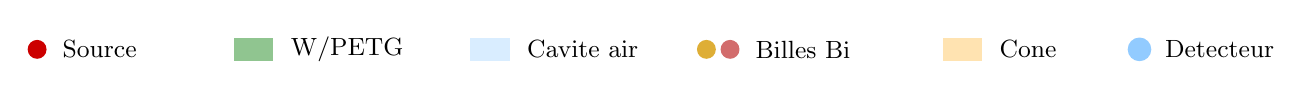
\begin{tikzpicture}[scale=1]
    \fill[red!80!black] (0, 0) circle (0.12);
    \node[right, font=\small] at (0.2, 0) {Source};
    
    \fill[wpetg!50] (2.5, -0.15) rectangle (3, 0.15);
    \node[right, font=\small] at (3.1, 0) {W/PETG};
    
    \fill[aircolor!70] (5.5, -0.15) rectangle (6, 0.15);
    \node[right, font=\small] at (6.1, 0) {Cavite air};
    
    \fill[billeA!90] (8.5, 0) circle (0.12);
    \fill[billeB!90] (8.8, 0) circle (0.12);
    \node[right, font=\small] at (9, 0) {Billes Bi};
    
    \fill[conecolor, opacity=0.5] (11.5, -0.15) rectangle (12, 0.15);
    \node[right, font=\small] at (12.1, 0) {Cone};
    
    \fill[watercolor!70] (14, 0) circle (0.15);
    \node[right, font=\small] at (14.2, 0) {Detecteur};
\end{tikzpicture}
\end{center}

\vspace{1cm}

% =============================================================================
% CALCULS
% =============================================================================
\section*{Calcul du demi-angle du cone}

\begin{minipage}{0.48\textwidth}
\subsection*{Donnees geometriques}
\begin{itemize}
    \item Position source : $z_s = 20$ mm
    \item Centre plaque : $z_{plaque} = 46.5$ mm
    \item Epaisseur cavite : $h = 8.53$ mm
    \item Face avant cavite : $z_c = 42.2$ mm
    \item Section cavite : $50 \times 50$ mm$^2$
    \item Rayon inscrit : $r = 25$ mm
\end{itemize}
\end{minipage}
\hfill
\begin{minipage}{0.48\textwidth}
\subsection*{Calculs}

Distance source $\rightarrow$ cavite :
\[ d = z_c - z_s = 42.2 - 20 = 22.2 \text{ mm} \]

Demi-angle du cone :
\[ \theta = \arctan\left(\frac{r}{d}\right) = \arctan\left(\frac{25}{22.2}\right) = \mathbf{48.4°} \]

Angle total : $2\theta = \mathbf{96.8°}$

Angle solide : $\Omega = 2\pi(1 - \cos\theta) = \mathbf{2.11}$ sr
\end{minipage}

\end{document}
